\title{Cellular automata: digital gate}
\date{}

\documentclass[12pt]{article}

\usepackage[italian]{babel}
\usepackage[T1]{fontenc}
\usepackage[utf8]{inputenc}
\usepackage{graphicx}
\usepackage{amsmath}
\usepackage{amssymb}
\usepackage{float}

\begin{document}
\maketitle
\newpage

\section{Introduzione}
L'\emph{assigment} prevede l'implementazione di una porta logica mediante l'uso di un automa cellulare, in questo caso è stata scelto di implementare la funzione \emph{OR}.

\section{Automa Cellulare}
L'automa cellulare è una struttura matematica che permette la computazione di calcoli anche elaborati mediante una serie di evoluzioni locali, in una griglia discreta di elementi.

Ad ogni iterazione si valuta l'intorno di ogni cella e lo stato della cella evolve in funzione di esso. 
Si definisce l'insieme finito $\mathbf{S}$ degli stati possibili e l'insieme $\mathbf{T}$ delle regole di transizione. ogni cella $A$ evolve in funzione di $(S,T,R) $ dove $R$ è il suo intorno.

\begin{figure}[h]
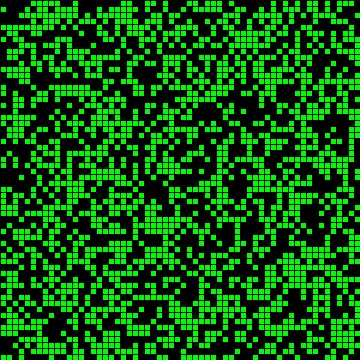
\includegraphics{Cellular_Automata.jpg}
\centering
\end{figure}

\section{Digital gate}
Allo scopo di simulare l'esecuzione della porta \emph{OR} è necessario scegliere un insieme di stati e regole adatti, gli stati sono:
\begin{itemize}
\item Empty
\item Conductor
\item Electron head
\item Electron tail
\end{itemize}
Che stanno ad indicare uno spazio vuoto, un elemento del conduttore, la testa e la coda dell'elettrone di passaggio. Gli ultimi due nomi non hanno un significato fisico ma permettono di semplificare intuitivamente la procedura.
Le regole di aggiornamento dello stato sono le seguenti:
\begin{itemize}
\item Empty $\rightarrow$ Empty
\item Conductor $\rightarrow$  $\lbrace$ Electron head,  Electron tail $\rbrace$
\item Electron head $\rightarrow$ Electron tail
\item Electron tail $\rightarrow$ Conductor
\end{itemize}
Il passaggio da \emph{Conductor} dipende dall'intorno dell'elemento, passa infatti a \emph{Electron head} se esattamente 1 o 2 delle celle dell'intorno sono nello stato di \emph{Electron head}, altrimenti resta nello stato di \emph{Conductor}.

Al fine di costruire la porta \emph{OR} è necessario inizializzare la griglia come in figura: 
\begin{figure}[h]
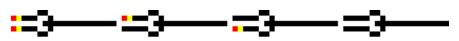
\includegraphics{Digital_gate.jpg}
\centering
\end{figure}
Le celle rosse rappresentano la coda dell'elettrone e le celle gialli la testa. Il nero, invece, rappresenta il conduttore.

\section{Risultati}
La transizione tra gli stati è stata rappresentata mediante \emph{ASCII art} ed è possibile notare il funzionamento coretto della computazione.


\end{document}
